\documentclass[10pt, twoside]{article}
\usepackage{zju-ds}
\usepackage{fontspec}

% 下面是用来设置填充示例内容的包, 可以删除
% The following packages are used to fill in the example content, which can be deleted
\usepackage[base]{babel}
\usepackage{lipsum}

% 是否为互评版本
% 会根据是否为互评自动屏蔽部分个人信息
% Controls whether to show personal information
% based on whether it is a peer review version.
\IsPRtrue  % 是互评版本
% \IsPRfalse % 非互评版本

% 报告标题
% Title
\newcommand{\reportname}{
    Advanced Data Structures\\
    and Algorithm Analysis\\
    Project Report}
\newcommand{\projectname}{
    Project Name
}

% 设置作者信息
% Author information
\newcommand{\authorname}{Author Name}
\newcommand{\authorID}{Author Stu. ID}

% 报告封面
% Title page
\title{
    \includesvg[scale=3]{assets/zju.svg}\\
    \ \\
    \textbf{\reportname}\\
    \projectname
    \ifIsPR (Peer Review) \fi
}

% 报告作者
% Author
\author{
    \ifIsPR
        ****\\
        **********
    \else
        \authorname\\
        \authorID
    \fi
}

% 设置页眉
% Set the header
\fancyhead[RO,LE]{\bfseries \thepage}
\fancyhead[RE]{\removelinebreaks{\reportname}}
\fancyhead[LO]{\projectname}

% 此处用于清除 PDF 文档属性中的身份信息
% Clear the identity information in the PDF document properties
\hypersetup{
    pdftitle={\ifIsPR \ \else \projectname \fi},
    pdfauthor={\ifIsPR \ \else \authorname \fi},
    pdfsubject={\ifIsPR \ \else \authorname \fi},
    pdfkeywords={\ifIsPR \ \else \reportname \fi},
    pdfcreator={\ifIsPR \ \else \authorname \fi},
    pdfproducer={\ifIsPR \ \else zjuds-template \fi},
}

% 文档开始
\begin{document}

% 设置 minted 代码显示风格
\setminted{
    fontsize=\normalsize,
    breaklines=true,
    style=manni,
    highlightcolor=Khaki1
}

% 封面页
\begin{titlingpage}
    \maketitle
    \thispagestyle{empty}
\end{titlingpage}
\newpage

% 正文内容
\section{Introduction}
\subsection{Background}

\lipsum[1]

\subsection{Detail Problem}

\lipsum[2-3]

\subsection{Input and Output Formats}

\lipsum[4]

\begin{center}

    \begin{tikzpicture}[>=Stealth, rainbow/.style={circle, draw, align=center, font=\bfseries, text=white, minimum size=1cm}]

        \def\numNodes{5}
        \def\numEdges{6}

        \foreach \i in {1,...,\numNodes}{
                \pgfmathsetmacro{\hue}{(\i-1)/(\numNodes-1)*120}
                \definecolor{currentColor}{RGB}{50, \hue, 150}
                \node [rainbow, fill=currentColor] (\i) at ({360/\numNodes * (\i - 1)}:2) {\i};
            }

        \foreach \source/\target/\weight in {
                3/4/130
            }{
                \draw[->, line width=0.8pt] (\source) -- node[midway, above, sloped, font=\footnotesize, color=black] {\weight} (\target);
            }

        \foreach \source/\target/\weight in {
                4/1/30,
                4/5/40
            }{
                \draw[->, color=bllue, line width=0.8pt] (\source) -- node[midway, above, sloped, font=\footnotesize, color=bllue] {\weight} (\target);
            }

        \foreach \source/\target/\weight in {
                1/5/40,
                2/4/80,
                3/2/60
            }{
                \draw[->, color=magenta, line width=0.8pt] (\source) -- node[midway, above, sloped, font=\footnotesize, color=magenta] {\weight} (\target);
            }
    \end{tikzpicture}

    \textbf{A Beautiful Graph, by tikz}
\end{center}

\section{Algorithm Specification}

\subsection{Algorithm}

\lipsum[19][2-6]

\subsubsection{Pseudo Code}

\begin{algorithm}[H]
    \caption{Conver to 3NF}
    \SetAlgoLined
    \KwData{$R$: a relation}
    \KwData{$F$: a set of functional dependencies}

    \While{there is a relation $R_i$ that is not in 3NF}{
        \ForEach{functional dependency $X \rightarrow Y$}{
            \If{$X$ is not a superkey of $R_i$}{
                Decompose $R_i$ into $R_i - Y$ and $X \cup Y$\;
            }
        }
    }
\end{algorithm}

\subsection{Data Structures and the Main Program}

\lipsum[8][1-7]

\subsubsection{Sketch of the main program}

\begin{figure}[!ht]
    \centering
    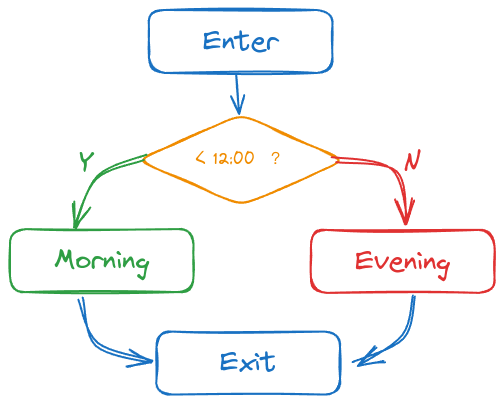
\includegraphics[width=0.4\linewidth]{assets/sketch.png}
    \caption{Sketch of the main program, by excalidraw}
\end{figure}

\section{Testing Results}

\subsection{Test method}

\lipsum[10-11]

\begin{table}[!ht]
    \centering
    \caption{Software Specification}
    \begin{tabular}{ccc}
        \toprule
        \textbf{Kernel} & \textbf{Compiler} & \textbf{Additional Compilation Option} \\
        \midrule
        Linux 6.10.9    & GCC 14.2.0        & \verb|-std=c11 -O2|                    \\
        \bottomrule
    \end{tabular}
\end{table}

\subsection{Test Cases}

\textbf{Case 1} Example case in the problem description:

\hspace{1cm}
\begin{minipage}[t]{0.3\textwidth}
    \textbf{Input}
    \begin{minted}[linenos=false]{text}
i
am
input #1
\end{minted}
\end{minipage}
\begin{minipage}[t]{0.2\textwidth}
    \textbf{Output}
    \begin{minted}[linenos=false]{text}
I AM OUTPUT #1
\end{minted}
\end{minipage}

\section{Analysis and Comments}

\subsection{Time complexity}

$O((M+N)^2 \log M)$, $\Omega((M+N)^2 \log M)$, $\Theta((M+N)^2 \log M)$.

\lipsum[4-6]


\subsection{Space compleixty}

\lipsum[2-5]

$O((M+N)^2 \log M)$, $\Omega((M+N)^2 \log M)$, $\Theta((M+N)^2 \log M)$.

\newpage

\section{Source Codes}

\subsection{Hello World Example}
\begin{minted}[frame=single]{c}
#include <stdio.h>
int main() {
    printf("Hello, World!\n");
    return 0;
}
\end{minted}

\textbf{Declaration}

I hereby declare that all the work done in this project titled
\textit{\projectname} is of my independent effort.

% ADS Version:
% We hereby declare that all the work done in this project titled 
% \textit{\projectname} is of our independent effort as a group.

% \textbf{Signature}

% \ifIsPR
%     Omitted in peer review.
% \else
%     \begin{figure}[H]
%         \centering
%         \includegraphics[width=0.25\linewidth]{assets/sign.png}
%     \end{figure}
% \fi

\end{document}